\section{Results and analysis}
\begin{frame}<beamer>{Outline}
    \tableofcontents[currentsection,currentsubsection]
  \end{frame}
 \begin{frame}{Results}
     \begin{itemize}
         \item{ \textbf{Neural Networks 1 (Net-1h)}
         }
         \item { Accuracy is 97.78\%} 
     \end{itemize}
     
		\begin{center}
		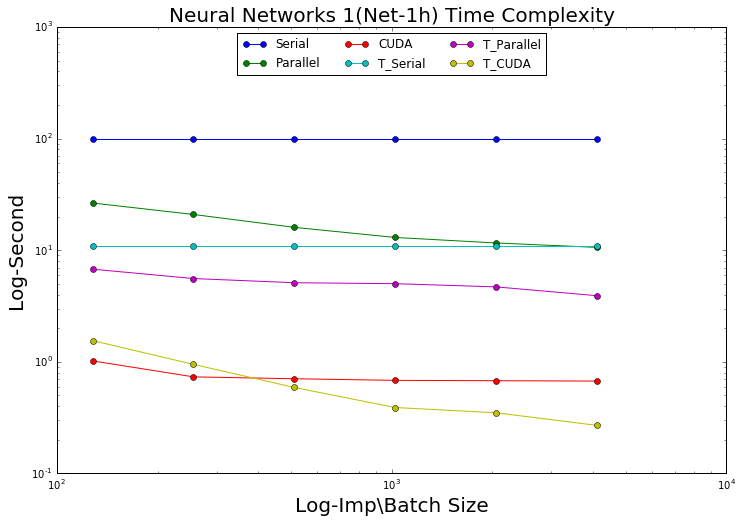
\includegraphics[width=3.4in]{nn1_time.png}
		\end{center}

 \end{frame}
 
\begin{frame}{Results (contd.)}
     \begin{itemize}
         \item{ \textbf{Neural Networks 2 (Net-2h)}
         }
         \item { Accuracy is ???\%} 
     \end{itemize}
     
		\begin{center}
		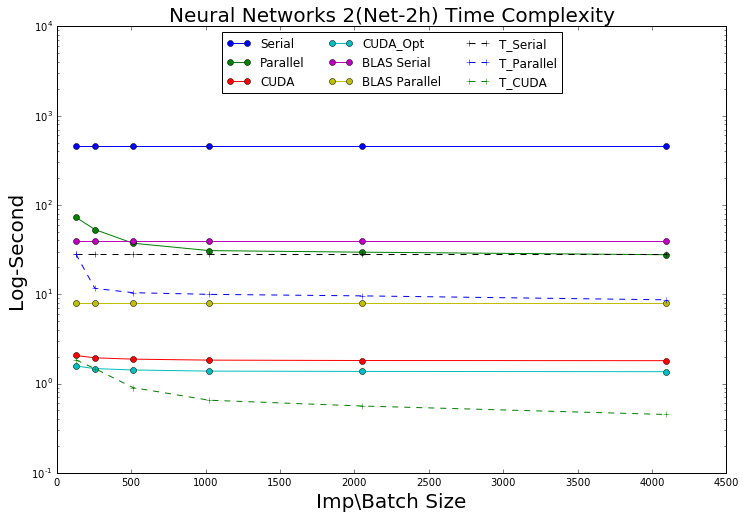
\includegraphics[width=3.4in]{nn2_time.png}
		\end{center}

 \end{frame} 

\begin{frame}{Results (contd.)}
     \begin{itemize}
         \item{ \textbf{Neural Networks 1 (Net-1h) - GFLOPS}
         }
     \end{itemize}
     
		\begin{center}
		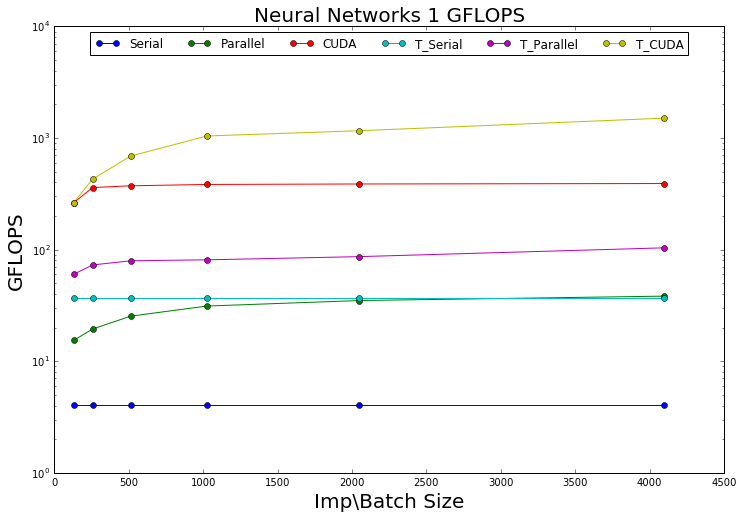
\includegraphics[width=3.4in]{nn1_gflops.png}
		\end{center}

 \end{frame} 

\begin{frame}{Results (contd.)}
     \begin{itemize}
         \item{ \textbf{Neural Networks 2 (Net-2h)- GFLOPS}
         }
     \end{itemize}
     
		\begin{center}
		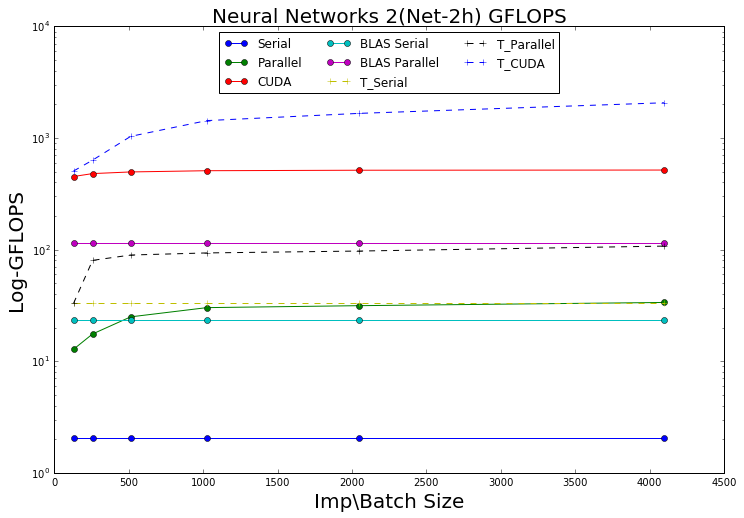
\includegraphics[width=3.4in]{nn2_gflops.png}
		\end{center}

 \end{frame} 

 
 \begin{frame}{Analysis}
 	\begin{itemize}
 	\item {Discussion}
 	\end{itemize}
 
 \end{frame}



